\documentclass[12pt, titlepage]{article}
\usepackage{graphicx}
\usepackage{booktabs}
\usepackage{ulem}
\usepackage{tabularx}
\usepackage{hyperref}
\usepackage{float}
\usepackage{color}
\usepackage{enumerate}
\hypersetup{
    colorlinks,
    citecolor=black,
    filecolor=black,
    linkcolor=red,
    urlcolor=blue
}
\usepackage[round]{natbib}

\title{SE 3XA3: Software Requirements Specification\\Asteroids War Game}

\author{Team \#12, Team Name
		\\ Student 1 Eric Thai Thaie1
		\\ Student 2 Tianzheng Mai and mait6
		\\ Student 3 Linqi Jiang and jiangl21
		\\ Student 4 Junhong Chen and chenj297
}

\date{\today}

\begin{document}
\begin{table}[bp]
\caption{\bf Revision History}
\begin{tabularx}{\textwidth}{p{3cm}p{2cm}X}
\toprule {\bf Date} & {\bf Version} & {\bf Notes}\\
\midrule
2/12/2021 & 1.0 Projec Drivers & Tianzheng Mai\\
2/12/2021 & 2.0 Functional Requirement & Junhong Chen\\
2/12/2021 & 3.0 Non-Functional Requirement & Eric Thai\\
2/12/2021 & 4.0 Project Issues & Linqi Jiang\\
4/12/2021 & Final Revision & Linqi Jiang\\
\bottomrule
\end{tabularx}
\end{table}
\newpage
\maketitle

\pagenumbering{roman}
\tableofcontents
\listoftables
\listoffigures



\newpage

\pagenumbering{arabic}

This document describes the requirements for Asteroid Game Development. The template for the Software Requirements Specification (SRS) is a subset of the Volere
template.  If you make further modifications
to the template, you should \sout{explicity}\textcolor{red}{explicitly} state what modifications were made.

\section{Project Drivers}

\subsection{The Purpose of the Project}
The goal of this project is to improve the user interface, functionality, and implementation of the old Asteroid Game. Improving the user interface of the original game can significantly enhance the user experience because the players will be able to play this game with better qualities. More importantly, this project also aims to improve the functionality and implementation by reproducing a two players mode and \sout{a rank system which provides a method for users to evaluate their game performance with others} \textcolor{red}{adjusting the internal parameters of the game system}.
\subsection{The Stakeholders}
The stakeholders include the clients, customers, other stakeholders. 
\subsubsection{The Client}
The clients are the professors, teaching assistants of Software Engineering 3XA3 who are responsible to supervise the project and keep track of the project process. 
\subsubsection{The Customers}
The intended customers are the public people who have an intermediate understanding of the English language, interests in Asteroid, and the ability to use a computer device, mouse, keyboard, and web browser. 
\subsubsection{Other Stakeholders}
Indirect Stakeholder: The indirect Stakeholders are all developers in team 3XA3 Lab3 Group12 who are responsible to develop, modify, maintain the Asteroid Game, and achieve all targets and requirements in SRS.  
\subsection{Mandated Constraints}
\subsubsection{Time Constraint}
The entire project must be completed and submitted by April 12th, 2021. 
\subsubsection{Cost Constraint}
There is no cost for this project because the required software and open-resource codes are free to use. 
\subsubsection{Product Constraint}
This product requires users to have the access to an efficient internet connection and a web browser with a computer, keyboard, and mouse.
\subsubsection{Knowledge Constraint}
The users must have an intermediate understanding of the English language and the basic knowledge to browser a website.

\subsection{Naming Conventions and Terminology}

\subsubsection{JavaScript}
A high-level, object-oriented computer programming language conforms to the ECMAScript specification. It is commonly used to create interactive effects in a web browser. 

\subsubsection{HTML}
Hypertext Markup Language (HTML) is the standard markup language for documents designed to be displayed in a web browser.

\subsubsection{CSS}
Cascading Style Sheets (CSS) is a style sheet language designed to enable the separation of presentation and content, including layout, colors, and fonts. 

\subsubsection{Node.js}
an open-source, cross-platform, back-end JavaScript runtime environment built on Chrome’s V8 JavaScript engine. 

\subsubsection{JSON}
JavaScript Object Notation (JSON) is an open file and data interchange format to store and transmit data objects consisting of attribute-value pairs and array data types.  


\subsection{Relevant Facts and Assumptions}

Asteroids will assume that the intended users must at least maintain an intermediate understanding of the English language and the ability to browse a website with using a computer, keyboard, and mouse. However, this application will not require the users to have any other technical background or education because a user manual will be provided on the main page of Asteroids.  

\section{Functional Requirements}

\subsection{The Scope of the Work and the Product}

\subsubsection{The Context of the Work}
Asteroids is a browser game in which the user can control a spaceship and shoot asteroids while avoiding getting hit by them. The context of the work is to rebuild and modify Asteroids, including editing the existing code for better readability and maintainability, improving the interface of the game by adding some colors and images,  \textcolor{red}{creating additional web pages such as user maunal and contact-us page, }adding some advanced features like score counting,\sout{difficulty level selection, leaderboard} and two-player mode.\\
Here are the deadlines and deliverables of the project:
\begin{itemize}
\item Project Approval~~~---Week of January 18
\item Problem Statement~~~---Week of January 25
\item Development Plan~~~ ---January 29
\item Requirements Docs Revision 0~~~ ---February 12
\item Proof of Concept Demonstration~~~---Week of February 22
\item Test Plan Revision 0~~~ ---March 5
\item Design and Document Revision 0~~~---March 18
\item Revision 0 Demonstration~~~---Week of March 22
\item Final Demonstration (Revision 1)~~~---Week of April 5
\item Final Demonstration (Revision 1)~~~---Week of April 12

\item 

\end{itemize}

\subsubsection{Work Partitioning}

\begin{table}[H]

		\centering
		\begin{tabular}{|c|c|c|c|}
			\hline
			Event Number& Event Name & Input & Output  \\ 
			\hline 
						1    &Asteroids Creation       &developer code     &web browser
          \\ 
			\hline 
						2  &User Interaction        &developer code      &web browser
        \\ 
			\hline 
						3  &Graphics Creation      &developer code     &web browser
       \\ 
			\hline 
						4  &Game Audio        &audio file      &sound effect
      \\
			\hline 
						5  &Asteroids Final Changes and Review        &developer code    &web browser
     \\ 
			\hline 
		\end{tabular} 
		\caption{Work Partitioning}
        \label{table:nonlin}
	\end{table}	

\newpage
\subsubsection{Individual Product Use Cases}
\begin{figure}[h]
	\centering
	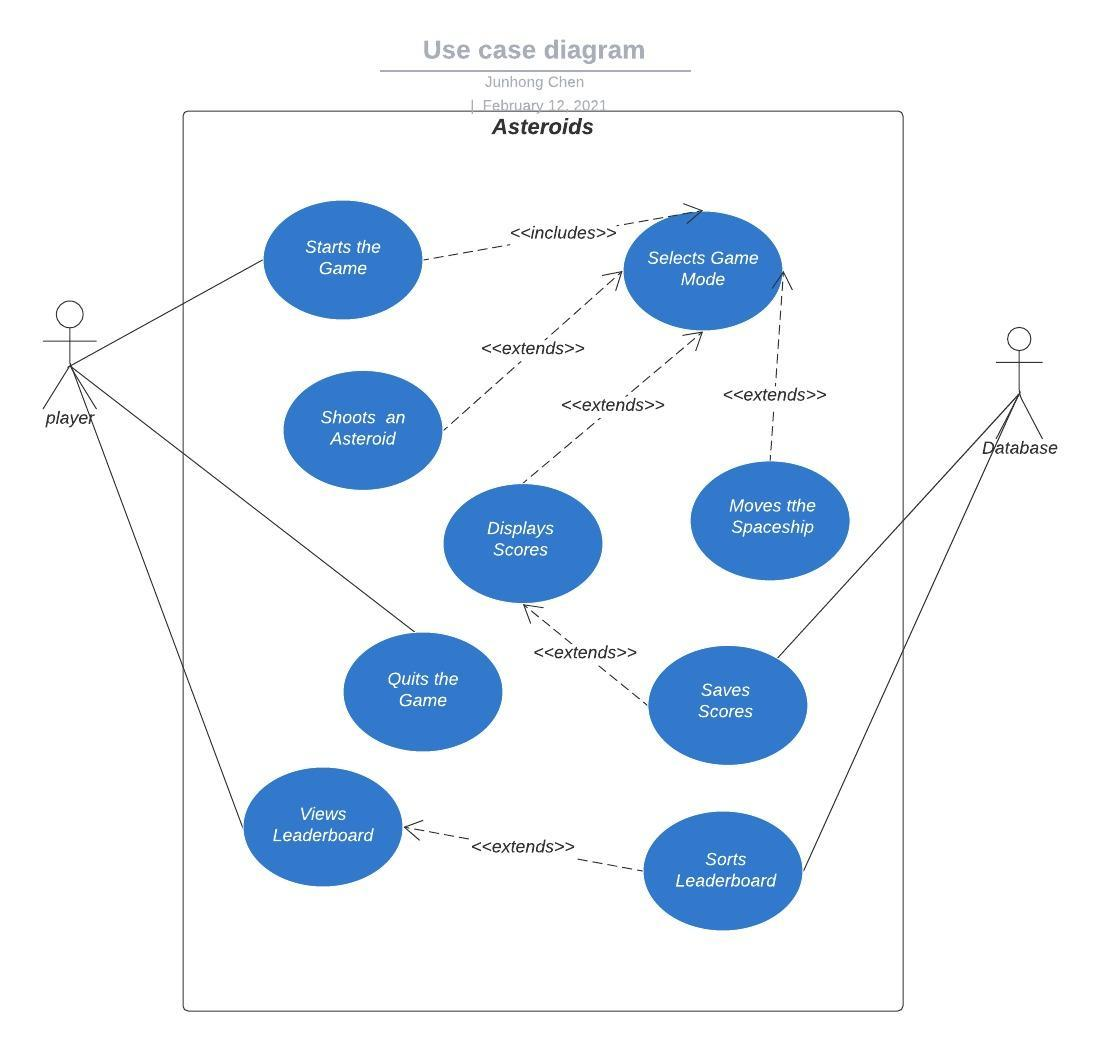
\includegraphics[width=1\textwidth]{use case diagram.jpg}
	\caption{Use Case Diagram for Asteroids}
	\label{cat 1}
\end{figure}

\subsection{Functional Requirements}
\begin{enumerate}[{FR}1.]
    \item The users must be able to access the website and play the game.\\
        Fit Criterion:  The user will be able to access the game by \sout{inputting the link to the web browser} \textcolor{red}{importing the game package and open the html files} \sout{and clicking the} \sout{start button} \textcolor{red}{ and pressing the Space key on the keyboard} to start the game.
        \item Scores should be shown on the screen to the users during the game. \\
        Fit Criterion: The game will display the scores that the player gains when playing the game.
		
		\item When the spaceship is hit by an asteroid, the lives of the spaceship will be reduced by 1.\\
        Fit Criterion: The lives of spaceships will be reduced by 1 when collision of it and an asteroid occurs.
        
        \item When the lives of the spaceship is zero, the game will be over and the result will be shown.\\
        Fit Criterion: The game will generate a result message and display the scores after the player loses three lives.
       
        \item The game will generate a battlefield for the player.\\
         Fit Criterion: The website interface will generate a battlefield that allows the user to control the spaceship to fly around in a limited size.

        \item The game will generate a spaceship for the player.\\
         Fit Criterion: The website interface will generate a spaceship that allows the user to control by arrow keys three lives and is able to shoot the asteroid to destroy them by pressing space.

        \item The main page of Asteroid will include a user manual for the player.\\
	Fit Criterion: The users could view the instructions and controls of the game by viewing the user manual. 

  \item \sout{ The game will include a stop button on the side. \\ Fit Criterion: The users can stop the game by clicking on the stop button.\\ }
	\textcolor{red}{The game will have a pause function.\\
	Fit Criterion: The users can pause the game by pressing the P key on the keyboard.}
	\item The battlefield interface must display the information of the spaceship.\\
         Fit Criterion: The battlefield will illustrate the spaceship information on the \sout{upper left corner} \textcolor{red}{upper right corner} which contains the spaceship lives and current scores.
        \textcolor{red}{\item The main page of Asteroid will include a contact-us page for the player.\\
	Fit Criterion: The users could view the contact information of our group members.}
		\textcolor{red}{\item The game will have the function of displaying the frame rate. \\ Fit Criterion: The users can press the F key on the keyboard to display the frame rate on the screen.}
\end{enumerate}

\section{Non-functional Requirements}

\subsection{Look and Feel Requirements}
\begin{enumerate}[\textcolor{red}{NFR-L}1.]

    \item The application must follow design standards and have a pleasant design.\\
\textcolor{red}{Fit Criterion: The codes follow the standards of programming languages that we use.}
    \sout{\\The application should draw user's in from its look.}
\end{enumerate}

\subsection{Usability and Humanity Requirements}
\begin{enumerate}[\textcolor{red}{NFR-U}1.]
    \item The application must be familiar to other browser games such that the controls are easy to use and learn.\\
   \textcolor{red}{Fit Criterion: Compare the interface of the game with other browser game which provides excellent user experience.}
    \item The application must be able to be used by users with a standard QWERTY keyboard.\\
     \textcolor{red}{Fit Criterion: User uses a standard QWERTY keyboard to play the game.}
    \item The application must provide instructions that can be understood by users that can read basic English.\\
      \textcolor{red}{Fit Criterion: User can access the user manual page to view the instructions.}
    \item The application must have a user interface that is friendly for those that are color blind.\\
\textcolor{red}{Fit Criterion: User who is blind can still see the game objects when playing the game.}  
    \item The user interface must follow web accessibility standards.\\
    \textcolor{red}{Fit Criterion: the html codes that we write follow the   standards of html.}  
\end{enumerate}

\subsection{Performance Requirements}
\begin{enumerate}[\textcolor{red}{NFR-P}1.]
    \item The application responds with very little to no latency.\\
\textcolor{red}{Fit Criterion: User will access the game on the browser in a very short time}
\end{enumerate}

\subsection{Operational and Environmental Requirements}
\begin{enumerate}[\textcolor{red}{NFR-O}1.]
    \item The application shall be able to run by opening an HTML file on a browser\\
\textcolor{red}{Fit Criterion: The User can access the game by open the HTML file, and the game will then be executed and displayed on the browser screen }
    \item The application will be usable on a standard web page size.\\
\textcolor{red}{Fir Criterion: The game screen will illustrated in a size which fit the screen}
\end{enumerate}
\subsection{Maintainability and Support Requirements}
\begin{enumerate}[\textcolor{red}{NFR-M}1.]
\item The application shall be able to run on the majority of the most popular web browsers\\
\textcolor{red}{Fit Criterion: Various of browser are accepted for this game including edge, google, Firefox. etc }
\item The application shall be able to run on Windows and MacOS\\
\textcolor{red}{Fir Criterion: Different system is also accepted for this game}
\end{enumerate}

\subsection{Security Requirements}
\begin{enumerate}[\textcolor{red}{NFR-S}1.]
    \item The Application's source code shall be open source.\\
    \textcolor{red}{Fit Criterion: The User can view the source code in src file, all the source code, png files and html files are arranged in it}
    \item Changes made to the application shall be traced back to the user who has made the changes\\
    \textcolor{red}{Fit Criterion: The application would be shown to the user in the source file}
\end{enumerate}

\subsection{Cultural Requirements}
\begin{itemize}
    \item None
\end{itemize}
\subsection{Legal Requirements}
\begin{enumerate}[\textcolor{red}{NFR-L}1.]
    \item The product shall comply with WCAG standards\\
    \textcolor{red}{Fir Criterion: User can check the source file with standard WCAGs, all the rules and principles are corrected}
    \end{enumerate}

\subsection{Health and Safety Requirements}
\begin{enumerate}[\textcolor{red}{NFR-H}1.]
    \item The application must not have flashing lights which could cause an epileptic user to experience a seizure\\
    \textcolor{red}{Fir Criterion: Our product is very healthy, there is no side effects but the user should notice the time of playing this game}
\end{enumerate}
\section{Project Issues}

\subsection{Open Issues}
The old game was initially implemented as a black and white rough interface. Our group will redesign the user interface and add some new features to the game so as to enhance the performance and quality of the game. 


\subsection{Off-the-Shelf Solutions}
\subsubsection{Existing Products}
There are many existing products for that have created the game of Asteroid, They are listed below:\\
Asteroid online game:\\
\url{http://www.dougmcinnes.com/html-5-asteroids}\\
Asteroid online scoreboard:\\
\url{https://games.aarp.org/games/atari-asteroids}\\
Improved classic Asteroid  game - webstore:\\
\url{https://chrome.google.com/webstore/detail/asteroids-classical-aster/pdjmcidindccobjfklphgnefglooeidl}\\


For this project, there are a lot of examples on the website, to create a better version of Asteroid, one of the important steps is to investigate these existing solutions, analyzing the advantages and drawbacks and improve the implementations and meet the project requirements.


\subsection{New Problems}
\subsubsection{Problems in System}
The project must be run on a web browser. The game will be interrupted and stop running if the system server crashes or the internet connection is lost. 
\subsubsection{Problems in Compiling Environment}
The game interface must be compatible with diverse devices and browsers which the users can play this game on different sizes of screen. 

\subsection{Tasks}
This is the link of Gantt Chart:\\
\url{https://gitlab.cas.mcmaster.ca/mait6/3xa3-lab3-group-12/-/blob/master/BlankProjectTemplate/ProjectSchedule/ganttchart.pdf}

\subsection{Migration to the New Product}

N/A

\subsection{Risks}
Testing is a risk on this project because it can not find out all potential errors which may be made in the development process. 


\subsection{Costs}
There is no cost in this game because the codes are open-resource and the software is free.

\subsection{User Documentation and Training}
N/A
\subsection{Waiting Room}
N/A
\subsection{Ideas for Solutions}

HTML and CSS will be used to improve the user interface. \\
JavaScript will be used to develop some new features and improve the functionality of the game. \\
JSON will be used to store and update the game data. \\


\bibliographystyle{plainnat}

\bibliography{SRS}

\newpage

\section{Appendix}

This section has been added to the Volere template.  This is where you can place
additional information.

\subsection{Symbolic Parameters}

The definition of the requirements will likely call for SYMBOLIC\_CONSTANTS.
Their values are defined in this section for easy maintenance.


\end{document}